\subsection{Pipes and Filters} \label{chp:pipes and filters}
Die höchste Abstraktion stellt das \first{Pipes and
Filters}-Patten dar
\footnote{
\textbf{Das Pipes and Filter Pattern}
	ist ein Architekturmuster für Systeme, die einen Strom von Daten verarbeiten.
	Jeder Verarbeitungsschritt ist in einen eigenen Filterkomponenten gekapselt.
	Die Daten werden dabei durch \name{Pipes} geleitet, die benachbarte
	\name{Filter} verbinden.
	Durch die Kapselung der Filter können diese frei kombiniert und
	getauscht werden, wodurch prinzipiell ähnliche, im Detail jedoch
	unterschiedliche Systeme entstehen.
	\citep{buschmann_pattern-oriented_1996}
}:
\index{Architekturmuster!Pipes and Filters}

\begin{figure}[htbp]
	\begin{center}
		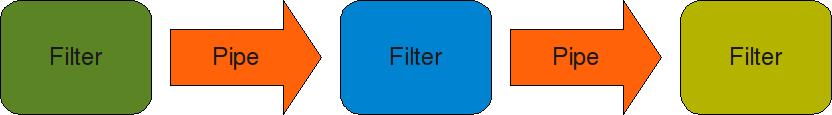
\includegraphics[scale=0.7]{pics/pipesFilter3.png}
	\caption[Pipes and Filter Pattern]{
	\textbf{Das Pipes and Filters Pattern.}
	}
	\end{center}
	\label{fig:pipesFilter}
\end{figure}

Die zu annotierende Sequenz wird schrittweise durch verschiedene \first{Filter}
bearbeitet. Jeder Filter, der in der \first{Pipeline} vorhanden ist, wird dabei
das entgültige Ergebnis der Annotation durch seine spezifischen Ergebnisse
erweitern.

Der Input eines Filters besteht dabei zum einen aus der zu
annotierenden Sequenz selbst, zum anderen aus einem zentralen Datenobjekt, in
dem alle gewonnenen Ergebnisse abgespeichert werden.
Ein Filter kann dabei auch auf die Ergebnisse eines anderen
Filters zugreifen oder auch angewiesen sein.
Die Reihenfolge der Filter innerhalb der Pipeline wird
somit durch die spezifischen \name{preconditions} \citep{beck_patterns_1994}
aller Filter festgelegt.
\index{Filter}

Es ist davon auszugehen, dass die Ausführung einzelner Filter mitunter sehr
zeitintensiv sein wird. Ausserdem soll Nutzen aus dem im Institut installierten
\first{LSF} \seec{chp:zielsetzung} gezogen werden. Daher wird eine rein
sequenzielle Abfolge der Filter, wie es das Entwursmuster suggeriert, vermieden werden.
Stattdessen kann die Ausführung einzelner Filter parallel erfolgen.
Sind zu einem Zeitpunkt die \name{preconditions} mehrerer Filter erfüllt,
werden diese sofort zur Ausführung gebracht.
\index{Platform LSF}

Die Pipeline soll möglichst leicht konfigurierbar sein und sich an
individuelle Bedürfnisse anpassen lassen.
Vor diesem Hintergrund soll die Pipeline die \name{Filter} dynamisch laden und
vollständig von den statischen \name{Pipes} entkoppeln.
Beim Starten der Pipeline soll diese an einem bestimmten Ort (lokales
Verzeichnis oder entferntes Repository) nach vorhandenen \name{Filtern} suchen
und diese in der Pipeline installieren.

Die \name{Filter} des \name{Pipes and Filters} Pattern sind somit aus der
eigentlichen Anwendung herrausgelöst. Sie sind über eine generische
Schnittstelle repräsentiert, deren Implementierung zur Kompilierzeit nicht
bekannt ist.

Vor der Hintergrund einer allgemeineren und von dem \name{Pipes and
Filters}-Pattern losgelösten Bezeichnung, sollen die \name{Filter} im folgenden
\first{Steps} genannt werden.

\begin{figure}[htbp]
	\begin{center}
		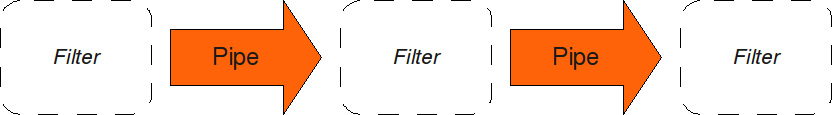
\includegraphics[scale=0.7]{pics/pipesFilter21.png}
	\caption[Dynamisches Pipes and Filter Pattern]{
	\textbf{Das dynamische Pipes and Filters Pattern.}
	Die Pipeline teilt sich in einen statischen (\name{Pipes}) und einen
	dynamischen Teil (\name{Filter}).
	Die \name{Filter} werden beim Programmstart von einem lokalen Verzeichnis oder
	einem entfernten Repository in das Programm geladen, wodurch die eigentliche
	Pipelinestruktur entsteht.
	}
	\end{center}
	\label{fig:pipesFilter21}
\end{figure}

